% !TeX spellcheck = cs_CZ
\section{Jednočinný propustný měnič}\label{ENZ:ssec_03}\hypertarget{ENZ:ssec_03} 
  Propustné měniče se vyznačují tím, že energie je přenášena ze vstupu na výstup v době zapnutí 
  tranzistoru, nikoli v době vypnutí, jak je tomu u měničů blokujících.
  
  V této i v následujících kapitolách budou analyzovány měniče typu DC/DC, které obsahují 
  vysokofrekvenční impulzní transformátor na feritovém jádře. Transformátor zajišťuje galvanické 
  oddělení mezi vstupní a výstupní stranou měniče. Je-li vstupní stejnosměrné napětí získáno 
  usměrněním střídavé sítě, pak bývají tyto měniče někdy označovány jako tzv. \emph{síťové 
  spínané 
  zdroje}.
  
  Celý výkonový řetězec sestává z následujících základních bloků:
  \begin{itemize}[noitemsep]
    \item buď síťový usměrňovač - stejnosměrný meziobvod - vlastní měnič,
    \item nebo akumulátor - stejnosměrný meziobvod - vlastní měnič.
  \end{itemize}
  
  Stejnosměrný meziobvod (ss. mezilehlý obvod, DC-bus, zwischenkreis) bývá napěťového typu, tj. 
  vůči následujícímu měniči se chová jako (téměř) ideální zdroj konstantního napětí \(U_d\) 
  nulovou vnitřní impedancí. Bývá realizován buď LC-filtrem, nebo samostatným sběracím 
  kondenzátorem o velké kapacitě. Dvojcestným usměrněním sítě 1 x \SI{230}{\volt} vznikne na 
  sběracím kondenzátoru ss. mezilehlé napětí \(U_d\) o hladině přibližně \SI{300}{\volt}. 
  Šestipulsním usměrněním sítě 3 x \SI{400}{\volt} vznikne ss. napětí o jmenovité střední hodnotě 
  \SI{542}{\volt}.
  
  Na hladině \SI{542}{\volt} se obvykle používají tranzistory IGBT se závěrným napětím 
  \SI{1200}{\volt}, které pracují na spínacím kmitočtu od \SI{25}{\kilo\hertz} do 
  \SI{60}{\kilo\hertz} (podle přenášeného výkonu). Kmitočet je ve většině případů omezen 
  především přepínacími ztrátami v tranzistorech IGBT.
  
  Na hladině \SI{300}{\volt} bývají převážně používány tranzistory MOSFET se závěrným napětím 
  \SI{600}{\volt}. Tranzistory jsou v současnosti tak rychlé, že mohou pracovat na spínacím 
  kmitočtu až do \SI{300}{\kilo\hertz}. Pracovní kmitočet ležívá typicky v oblasti 
  \SI{40}{\kilo\hertz} až \SI{120}{\kilo\hertz}. Jediným důvodem ke zvyšování kmitočtu je 
  zmenšování objemu transformátoru i výstupní tlumivky. Zvyšování kmitočtu nad 
  \SI{200}{\kilo\hertz} není výhodné z následujících důvodů:
  \begin{itemize}[noitemsep]
    \item Mezní kmitočet manganato-zinečnatých feritů leží kolem \SI{450}{\kilo\hertz}, tudíž 
          v pásmu nad \SI{200}{\kilo\hertz} prudce rostou hysterezní ztráty (viz komplexní 
          permeabilita v kap. 6.4.4.). Ztráty je nutno omezovat snižováním maximální pracovní 
          indukce \(B_{max}\), což působí proti zmenšování transformátoru.
     \item V oblasti nad \SI{200}{\kilo\hertz} začínají narůstat problémy se skinefektem ve  
          vinutí transformátoru (nikoli ve vinutí tlumivky, v ní je proud téměř hladký). Na 
          kmitočtu \SI{200}{\kilo\hertz} činí hloubka vniku již pouze \(\delta\cong\) 
          \SI{0,14}{\mm}, viz kap. 4. Nutné je použití vf. lanka nejen na sekundám (málo závitů a 
          velký průřez), ale i na primáni (více závitů a menší průřez). Výsledkem je pokles 
          činitele plnění ve vinutí, který působí proti zmenšování transformátoru.
    \item S rostoucím pracovním kmitočtem/dramaticky roste reaktance \(2\pi f L_{2,K}\) 
          výstupní rozptylové indukčnosti transformátoru \(L_{2,K} = L2(1 - k^2)\). Transformátor 
          je pak velmi měkký a není schopen přenést požadovaný výkon. Jedinou obranou je dosažení 
          co největšího činitele vazby \(k\). Hodnota \(k = 0,990\) je naprosto nedostatečná. 
          Nutným minimem bývá \(k = 0,998\), což ale přináší značné konstrukční problémy (viz 
          kap. 17.6).
    \item S rostoucím kmitočtem roste negativní vliv parazitních mezizávitových kapacit vinutí.
  \end{itemize}
  
  \subsection{Můstkový jednočinný propustný měnič - základní zapojení}
    Základní zapojení jednočinného propustného měniče s transformátorem je nakresleno na obr. 
    \ref{enz:fig_fey_1cinprop_m}. Jak již bylo předesláno, k přenosu energie ze vstupního do 
    výstupního obvodu dochází v aktivním intervalu \(0\) až \(\delta T\), během něhož se současně 
    akumuluje energie v magnetickém poli tlumivky \(L\). Po dobu zbývající části periody 
    $(1-\delta)T$ je tlumivka od transformátoru oddělena a na výstup dodává energii nahromaděnou  
    v magnetickém poli. Vzhledem k \emph{blokujícímu měniči} je zde výhoda účinného LC filtru 
    tvořeného tlumivkou a výstupním kondenzátorem \(C\) po dobu celého pracovního cyklu. Ve 
    srovnání s blokujícím měničem je tedy možné dosáhnout řádově menší dynamické odchylky 
    \(\Delta U_z(t)\). Navíc proud tekoucí \(L\), skládající se z ustálené složky $I_z$ a 
    pilovitého průběhu $\Delta i_L$ má spojitý charakter v průběhu celé periody $T$. 
    
    Časové průběhy všech důležitých veličin jsou zachyceny na obr. \ref{enz:fig_fey_1cinprop_mw}. 
    Z důvodu snadnějšího výkladu budeme při prvotní analýze předpokládat následující zjednodušení:

    \begin{itemize}[noitemsep]
      \item Tlumivka výstupního LC-filtru má velikou (nekonečnou) indukčnost. Proud tlumivky  
            \(i_L\) je hladký, málo zvlněný, tudíž je přímo roven proudu zátěže: \(i_L(t) = I_Z = 
            \text{konst}\).
      \item Transformátor má dokonalou magnetickou vazbu \(k=1\). Neexistuje tedy výstupní 
            rozptylová indukčnost \(L_{2,K}\).
    \end{itemize}
    Obě zjednodušení později při detailní analýze odstraníme.
    
    \begin{figure}[ht!]
      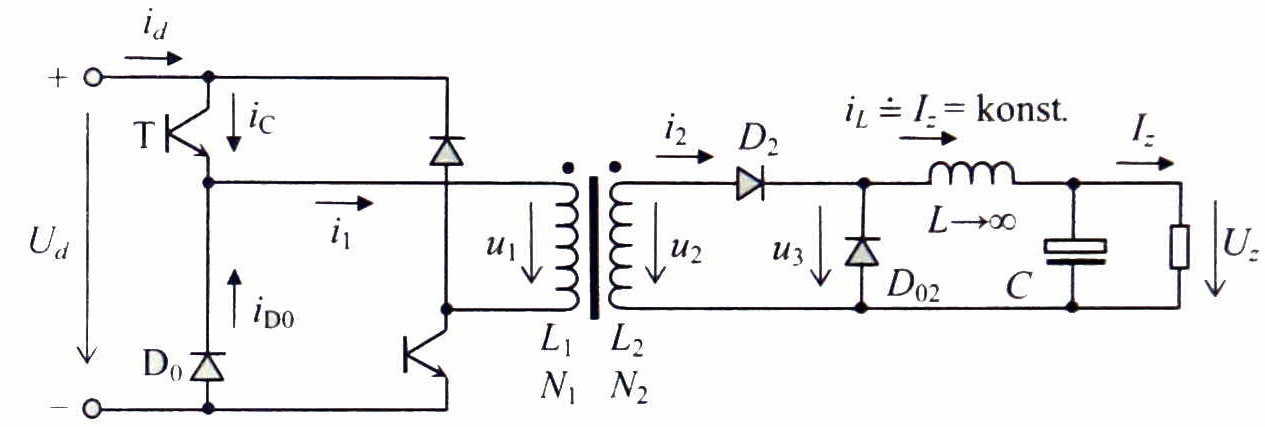
\includegraphics[width=\linewidth]{patocka_1cinprop_menic.JPG}
      \caption{Jednočinný propustný měnič - základní zapojení}
      \label{enz:fig_fey_1cinprop_m}
    \end{figure}
  
    Měnič pracuje tak, že oba tranzistory jsou vždy zapínány i vypínány současně. Doba zapnutí je 
    označena \(t_z\). Střída je definována vztahem
    \begin{equation}\label{enz:eq_1cinpropm01}
      s = \frac{t_z}{T}, \qquad s_{max} = \frac{1}{2}, \qquad \text{protože} \qquad t<\frac{T}{2}
    \end{equation}     

    \begin{figure}[ht!]
      \centering
      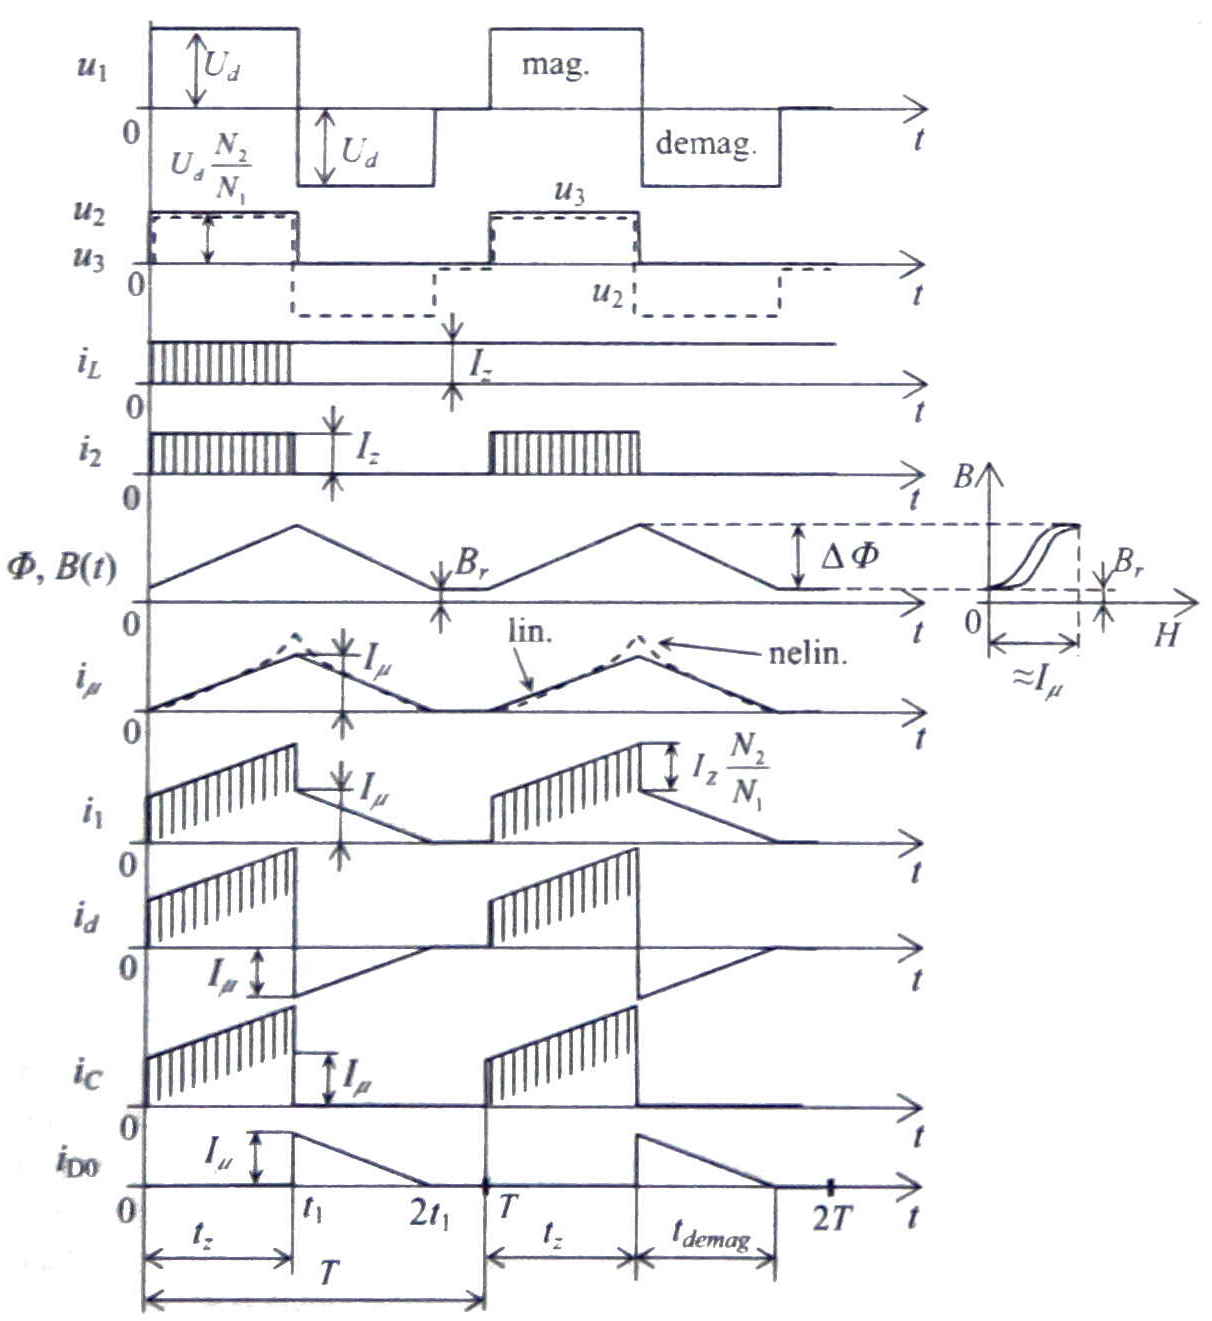
\includegraphics[width=\linewidth]{patocka_1cinprop_menic_w.JPG}
      \caption{Jednočinný propustný měnič - průběhy důležitých veličin.}
      \label{enz:fig_fey_1cinprop_mw} 
    \end{figure}
    
    Maximální doba zapnutí \(t_z=t_1\), nesmí překročit hodnotu \(\dfrac{T}{2}\), neboť pak 
    dochází k lavinovitému přesycení transformátoru podle obr. \ref{enz:fig_fey_1cinprop_syc}. 
    Při zapnutí obou tranzistorů má primární napětí konstantní hodnotu \(U_1(t)=+U_d\). 
    Magnetizační proud je integrálem z tohoto \emph{konstantního} napětí, proto narůstá 
    \emph{lineárně} (pokud zanedbáme nelinearitu magnetizační charakteristiky). V okamžiku 
    \(t_1\) jsou oba tranzistory vypnuty. Magnetizační indukčnost \(L_1\), však nedovolí zánik 
    magnetizačního proudu a snaží se jej udržet na původní velikosti. Proud tedy musí začít téci 
    oběma primárními diodami. Přes obě sepnuté diody připojí primární vinutí samo sebe na 
    napájecí zdroj \(U_d\) ale v opačné polaritě, tedy bude \(U_1(t)=-U_d\). Tímto napětím je 
    jádro \emph{demagnetováno} a magnetizační proud klesá, protože integrál ze záporné konstanty 
    je klesající přímka. Obě diody se uzavřou až v okamžiku zániku magnetizačního proudu. Teprve 
    tehdy je primární vinutí zcela odpojeno od mezilehlého zdroje \(U_d\), stává se neutrálním 
    vodičem neobsahujícím energii, proto teprve tehdy klesne primární napětí na nulu.
    
    Sekundární napětí \(u_2\) musí mít \emph{stejný tvar} jako napětí \(u_1\), pouze je s 
    převodem jinak velké. Záporný demagnetizační puls nesmí být využit k přenosu energie. Došlo 
    by k narušení procesu demagnetizace. Proto musí být na sekundáru použit pouze jednocestný 
    usměrňovač \(D_2\) s nulovou diodou \(D_{02}\) (nikoli dvojcestný). Dioda \(D_{02}\) vede 
    proud tlumivky v době, kdy jsou oba tranzistory vypnuty, a usměrňovači dioda \(D_2\) je 
    polarizována v závěrném směru. Užitečné napětí \(u_3\), na vstupu LC-filtru má potom tvar 
    jednopolaritních impulsů o maximální střídě 0,5.
    
    Sekundární proud \(i_2\) má podobu \emph{pravoúhlých} proudových impulsů, protože pokud proud 
    sekundárem teče, tlumivka s velikou indukčností \((L\rightarrow\infty)\) jej udržuje 
    \emph{konstantní}. S ohledem na vysoký pracovní kmitočet a na velký obsah harmonických je 
    nutno učinit velmi přísná opatření proti vzniku skinefektu. Z toho důvodu nesmí být průměr 
    sekundárního vodiče nebo tloušťka měděné fólie větší než \(2\delta\), kde \(\delta\) je 
    hloubka vniku. Totéž platí i o primárním vodiči.


    \begin{figure}[ht!]
      \centering
      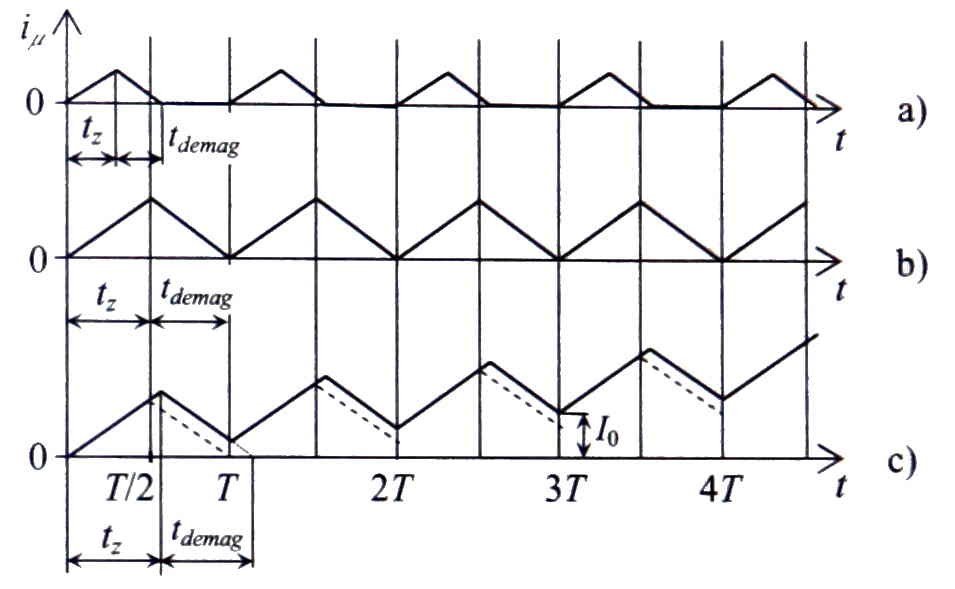
\includegraphics[width=0.8\linewidth]{patocka_1cinprop_syceni.JPG}
      \caption{Demagnetizace transformátoru při různých dobách zapnutí \(t_z\): a) dobrý stav 
               \(t_z < \frac{T}{2}\), b) mezní stav \(t_z = \frac{T}{2}\), c) špatný stav \(t_z > 
               \frac{T}{2}\)}.
      \label{enz:fig_fey_1cinprop_syc}
    \end{figure}
    Maximální doba zapnutí \(t_z=t_1\), nesmí překročit hodnotu \(\dfrac{T}{2}\), neboť pak 
    dochází k lavinovitému přesycení transformátoru podle obr. \ref{enz:fig_fey_1cinprop_syc}.  
    Jev je způsoben tím, že doby magnetizace a demagnetizace jsou stejně dlouhé, tj. 
    \(t_z=t_{demag}\). Demagnetizační proud proto zaniká v okamžiku \(2t_z\). Pokud v případě c) 
    doba zapnutí překročí \(\dfrac{T}{2}\), tj. \(2t_z > T\), magnetizační proud nestihne v rámci 
    pracovního cyklu \(T\) klesnout na nulu. Demagnetizace tudíž není dokončena. Tokotvorný 
    magnetizační proud \(i_\mu=I_0 + \frac{1}{L}\int{u_1\dd{t}}\) je pak integrován z nenulové 
    počáteční podmínky \(I_0\), která se při každém následujícím cyklu zvyšuje. Proto  proud 
    makroskopicky postupně narůstá do nekonečna. Ve skutečnosti se zastaví na veliké zkratové 
    hodnotě \(\dfrac{U_d}{R_{Cu1}}\). Podobně roste i magnetický tok. Jádro se tedy silně 
    přesycuje, klesá jeho indukčnost a o to rychleji lavinovitě roste magnetizační proud. 
    Výsledkem je velmi rychlá tepelná destrukce primárního vinutí (během několika sekund).      

  %------------- Návrh transformátoru ------------------------------------------------------------
  \subsection{Návrh transformátoru}
    
  %------------- Jednočinný propustný měnič s demagnetizačním vinutím ----------------------------
  \subsection{Jednočinný propustný měnič s demagnetizačním vinutím}
    
    \luagraphic[1]{aes_fig074.pdf}{Propustný měnič s akumulační tlumivkou  a demagnetizačním
    vinutím}{aes:fig074}
    
  \subsection{Popis činnosti}\label{ENZ:kap_forward_converter_describe}
    Nyní se věnujme podrobnějšímu rozboru funkce propustného měniče. Interval $\delta T$ začíná
    \textbf{sepnutím tranzistoru} $T_1$ kladným impulzem z řídicích obvodů do jeho báze     
    \cite[s.~131]{Hammembauer}, které přivede vstupní napětí na primární vinutí $N_1$. V kapitole
    \ref{ES:kap_rozbor_trafa} byl odvozen vztah \ref{es_eq_int_uprim_max} pro magnetizační tok v 
    jádře transformátoru. Pro nynější případ platí $u_1(t) = U_{in}$. Pak 
    \ref{es_eq_int_uprim_max} nabude tvaru 
    \cite[s.~104]{Patocka}:
    
    \begin{equation}\label{ENZ:eq_forward_phi_mag}
     \Phi_\mu(t)=\frac{1}{N_1}U_{in}t
    \end{equation}
    
    Takže po zapnutí tranzistoru tok lineárně narůstá (z nulové počáteční hodnoty). Na konci doby 
    zapnutí $\delta T$ bude mít své maximum 
    \begin{equation}\label{ENZ:eq_forward_phi_max}
     \Phi_{\mu_{max}}=\frac{1}{N_1}U_{in}\delta T
    \end{equation}
    Během doby $\delta T$ bude sekundární napětí $u_{2}(t)$:
    \begin{equation}\label{ENZ:eq_forward_usec}
     u_{2}(t) = N_2\frac{\Phi_\mu(t)}{dt} = \frac{N_2}{N_1}U_{in} = U_{2}
    \end{equation}
    Čili během doby $\delta T$ je sekundární napětí konstantní. Protože jde o kladné napětí, je 
    $D_1$ otevřená, $D_2$ zavřená a výstupní proud $I_{out}$ musí téci ze sekundárního vinutí 
    transformátoru.
    
    Kolektorovým obvodem a primárním vinutím $N_1$ teče proud $i_{prim}$. Propustně polarizovanou 
    diodou $D_1$ prochází transformovaný vstupní proud přes $L_{out}$ do zátěže a výstupního 
    filtračního kondenzátoru $C_{OUT}$. Tento sekundární proud $i_2$ se časem lineárně zvětšuje  
    od určitého $I_{L_{min}}$ a zároveň se lineárně zvětšuje také proud $i_1$, závislého na 
    převodu transformátoru. Z kapitoly \ref{ES:kap_rozbor_trafa} víme, že primární proud 
    zatíženého transformátoru bude mít hodnotu
    \begin{equation}\label{ENZ:eq_forward_iprim}
    i_1(t) = i_\mu(t) + I_2\frac{N_2}{N_1}
    \end{equation} 
    
    Pro magnetizační proud $i_\mu(t)$ přitom platí vztah (\ref{es_eq_imag_u1}). V našem případě je
    $u_1(t)=U_{in}$ a proto tento vztah dostane konkrétní podobu:
    \begin{equation}\label{ENZ:eq_forward_imagt}
     i_\mu(t) = \frac{U_1t}{L_1}
    \end{equation}
    Vidíme, že stejně jako tok $\Phi_\mu(t)$ tak i magnetizační proud $i_\mu(t)$ lineárně narůstá 
    (z nulové počáteční hodnoty). Na konci $\delta T$ má magnetizační proud své maximum:
    \begin{equation}\label{ENZ:eq_forward_imag_max}
     i_{\mu_{max}}(t) = \frac{U_1\delta T}{L_1}
    \end{equation}
    Během doby $\delta T$ je odebírána energie ze zdroje $U_{in}$ (složka $I_{out}\frac{N2}{N1}$
    primárního proudu) a dodávána do zátěže.
    
    Nyní vypneme tranzistor $T_1$. Proud $i_1(t)$ musí téměř skokem zaniknout. V jádře ale 
    existuje na konci doby $\delta T$ magnetický tok $\Phi_{\mu_{max}}$, odpovídající proudu 
    $I_{\mu_{max}}$. Celková energie magnetického pole v okamžiku vypínání tranzistoru činí 
    $\frac{1}{2}L_1I_{\mu_{max}}$. Proud primárního vinutí je tranzistorem násilně přerušen.
    
    Předpokládejme nejdříve, že neexistuje demagnetizační vinutí $N_3$. Pak by při skokovém zániku
    primárního magnetizačního proudu stejně prudce zanikl i s ním svázaný tok $\Phi_{\mu_{max}}$. 
    Pokles toku s obrovskou (teoreticky nekonečnou) strmostí $-\frac{d\Phi}{dt}$ způsobí vznik 
    napěťového Diracova impulsu, opačné polarity oproti stavu v době $\delta T$, kdy tok 
    narůstal. Tímto impulsem, přičteným k napětí $U_1$, je napěťově namáhán zavírající se 
    tranzistor. Přitom se celá energie $\frac{1}{2}L_1I_{\mu_{max}}$ přemění na křemíkovém čipu v 
    teplo a je příčinou jeho neodvratné destrukce. U reálného tranzistoru je velikost napěťového 
    impulsu vždy omezena průrazným napětím tranzistoru. Nikdy totiž není tranzistor natolik 
    pomalý, že by omezujícím faktorem byla malá strmost $-\frac{di_C}{dt}$ zániku kolektorového 
    proudu během vypínání. Destrukční energetické účinky však zůstávají v každém případě zcela 
    ekvivalentní.              
    
    Aby popsaná situace nenastala, je zde demagnetizační vinutí $N_3$. Děj pak bude vypadat 
    takto: Po vypnutí tranzistoru $T_1$ se opravdu na primárním vinutí objeví napětí $U_1'$ 
    opačné polarity, než bylo $U_1$ v sepnutém stavu, viz. obr. \ref{enz:fig_Forward_demag_wave}. 
    Toto napětí však bude mít přesně definovanou velikost, kterou „dovolí“ vinutí N3. Na tom se 
    totiž objeví také indukované napětí $u_3$. Vzhledem k obrácené orientaci vinutí vůči $N_1$ 
    bude mít záporný pól „na zemi“ a kladný pól na diodě $D_2$. Toto napětí by „chtělo“ být opět 
    teoreticky nekonečné, ale $D_2$ se otevře a pracuje v součinnosti se zdrojem  $U_1$ jako 
    napěťový omezovač, omezující napětí $u_3$ na velikost $U_1$. Celá magnetizační energie 
    $\frac{1}{2}L_1I_{\mu_{max}}$ je vinutím  $N_3$ odevzdána zpět do zdroje. Pak je zřejmé, že 
    napětí indukované v primárním vinutí musí být:
    
    \begin{figure}[ht!]
      \centering
      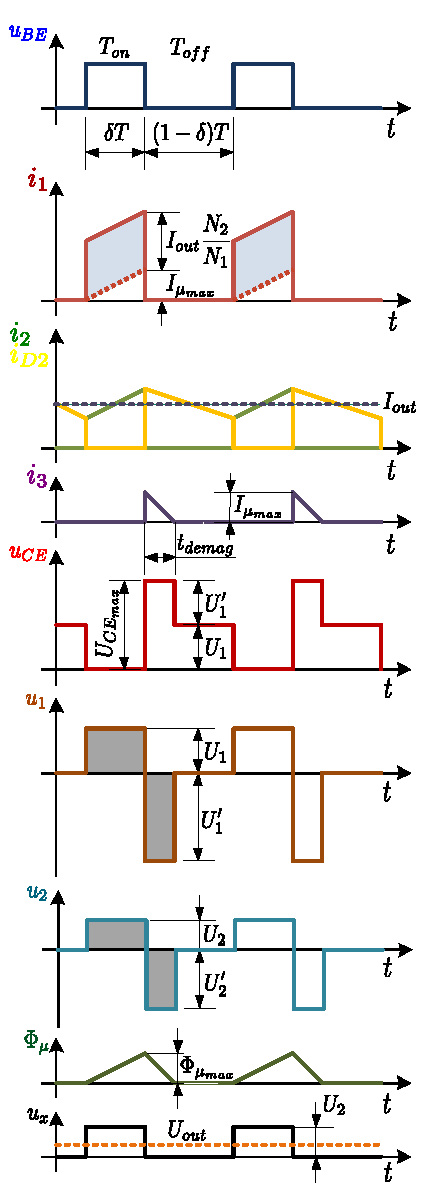
\includegraphics[width=0.7\linewidth]{Forward_converter_wave.pdf}
      \caption{Průběhy veličin propustného měniče s akumulační tlumivkou a demagnetizačním 
      vinutím}
      \label{enz:fig_Forward_demag_wave} 
    \end{figure}                          
    
    \begin{equation}\label{ENZ:eq_forward_u1_demag}
     U_1'=u_3\frac{N_1}{N_3} = U_1\frac{N_1}{N_3}
    \end{equation}
    Tento stav, kdy  $u_1 = -U_1$ a  $u_3 = U_1$, trvá po dobu, než tok $\Phi_\mu(t)$ klesne z 
    počáteční hodnoty $\Phi_{\mu_{max}}$ na nulu. K tomu je třeba konečné doby $t_{demag}$, neboť 
    $U_1$ není nekonečné a proto strmost poklesu $\frac{d\Phi}{dt}$ nemůže být nekonečně velká. 
    Velikost $U_1$ je v této době konstantní a proto klesá tok lineárně. Celý jev se nazývá 
    \emph{demagnetizací jádra}.
    
    Během demagnetizace se předává magnetizační energie jádra zpět do zdroje pomocí proudu 
    $i_3(t)$. Proud $i_3(t)$ je přímo úměrný klesajícímu toku $\Phi_\mu(t)$ takto:
    \begin{equation}\label{ENZ:eq_imag_phi_forward}
     i_3(t) = \frac{1}{L_3}\int{u_3}dt = \frac{1}{L_3}\int{\frac{N_3d\Phi_\mu(t)}{dt}}dt =
     \frac{N_3\Phi_\mu(t)}{L_3}
    \end{equation}
    Po skončení demagnetizace (uplynutí $t_{demag}$) je již magnetický tok nulový, jádro je 
    energeticky neutrální, proto i napětí $u_1$, $u_2$, $u_3$ skokem zanikají na nulu. V 
    neutrálním stavu soustava setrvává až do skončení doby $(1-\delta)T$, tj. do zapnutí 
    tranzistoru.
    
    Pro magnetický tok během procesu demagnetizace musí platit:
    \begin{equation}\label{ENZ:eq_phi_mag_forward}
     \Phi_\mu(t) = \Phi_{\mu_{max}} - \frac{\int{u_1(t)dt}}{N_1} = \Phi_{\mu_{max}} -
     \frac{U_1't}{N_1}
    \end{equation}
    Po uplynutí $t_{demag}$ je tok nulový. Položíme-li tedy $\Phi_\mu(t)$ dle
    (\ref{ENZ:eq_phi_mag_forward}) rovný nule, lze odsud vyjádřit $t_{demag}$.
    \begin{equation}\label{ENZ:eq_tdemag_forward}
     t_{demag} = \frac{N_1\Phi_{\mu_{max}}}{U_1'}
    \end{equation}
    Za $\Phi_{\mu_{max}}$ dosadíme vztah (\ref{ENZ:eq_forward_phi_max}) a za $U_1$  vztah
    (\ref{ENZ:eq_forward_u1_demag}). Tím dostaneme:
    \begin{equation}\label{ENZ:eq_tdemag_N1N3_forward}
     t_{demag} = \frac{N_3}{N_1}\delta T
    \end{equation}
    Je zřejmé, že musíme zajistit, aby $(1-\delta)T > t_{demag}$, jinak by tok ještě nestačil
    úplně zaniknout a už bychom znovu spínali tranzistor. V průběhu dalšího sepnutí by se tok (a
    magnetizační proud) zvýšil opět o hodnotu $\Phi_{\mu_{max}}$ (resp.  $I_{\mu_{max}}$, ale už z
    nenulové počáteční hodnoty a tak by neustále vzrůstal (během dalších period by se
    „naintegroval“ teoreticky na hodnotu $\rightarrow\infty$), až by došlo k přesycení jádra a tím
    k prudkému lavinovitému růstu magnetizačního proudu (neboť by současné klesla indukčnost
    $L_1$). Jev by postupoval až do zničení tranzistoru. Z výše uvedeného důvodu musí být
    maximální střída $\delta$ omezena na hodnotu:
    \begin{equation}\label{ENZ:eq_forward_delta_max}
    \delta_{max} = \frac{t_{on}}{t_{on}+t_{demag}}
    \end{equation}
    Dosazením (\ref{ENZ:eq_tdemag_N1N3_forward}) za $t_{demag}$ dostaneme:
    \begin{equation}\label{ENZ:eq_forward_delta_max1}
    \delta_{max} = \frac{N_1}{N_1+N_3}
    \end{equation}
    Výstupní napětí $U_{out}$ je rovno \emph{střední hodnotě napětí} $u_X$ a platí proto:
    \begin{equation}\label{ENZ:eq_uout_forward_delta}
    U_{out} = U_1\frac{N_2}{N_1}\frac{t_{on}}{t_{on} + t_{off}} = U_1\frac{N_2}{N_1}\delta
    \end{equation}
    
   %---------- Proudové a napěťové dimenzování součástek -----------------------------------------
  \subsection{Proudové a napěťové dimenzování součástek}
    V době $t_{demag}$ je tranzistor namáhán napětím $U_{{CE}_{max}}$:
    \begin{equation}\label{ENZ:eq_dim_Ucemax}
      U_{{CE}_{max}} = U_1 + U_1' = U_1 + \frac{N_3}{N_1}U_1 = U_1\frac{N_1+N_3}{N_1}
    \end{equation}
    \begin{itemize}[noitemsep]
     \item Volíme-li $N_3 < N_1$, je $U_1' > U_1$ a tedy namáhání $U_{{CE}_{max}} > 2U_1$. Zato
           je ale maximální dovolená střída $\delta_{max} > 0,5$ a je tedy větší maximální
           dosažitelné výstupní napětí.
     \item Volíme-li $N_3 > N_1$, je $U_1' < U_1$ a je tedy  $U_1 < U_{{CE}_{max}} < 2U_1$. Zato
           je ale maximální dovolená střída $\delta_{max} < 0,5$ a je tedy menší maximální
           dosažitelné výstupní napětí.
    \end{itemize}
    Volba  poměru  $N_3/N_1$ proto záleží na tom, co je v dané aplikaci více kritické, zda
    napěťové namáhání tranzistoru,  či co největší dosažitelné výstupní napětí (s neměnným
    převodem  $N_2/N_1$). V praxi se nejčastěji volí $N_3 = N_1$ z důvodů snadného souběžného
    (\emph{bifilárního}) vinutí obou cívek - viz později.
    
    \begin{itemize}
      \item \emph{Proudové a dimenzování $T_1$:}
         \newline Zanedbáme-li magnetizační proud, pak lze psát, viz. obr.
         \ref{enz:fig_Forward_demag_wave}, pro špičkovou, střední a efektivní hodnotu
         kolektorového proudu tranzistoru následující rovnice:
          \begin{align}
              I_{1_{max}} &= I_{out}\frac{N_2}{N_1}             \\
              I_{1_{av}}  &= I_{out}\frac{N_2}{N_1}\delta       \\
              I_{1_{rms}} &= I_{out}\frac{N_2}{N_1}\sqrt{\delta}
          \end{align}
      \item \emph{Proudové a napěťové dimenzování $D_1$:}
          \begin{align}
              I_{D_{1max}} &= I_{out}                \\
              I_{D_{1av}}  &= I_{out}\delta          \\
              I_{D_{1rms}} &= I_{out}\sqrt{\delta}   \\
              U_{D_{1Rmax}}&= U_1\frac{N_2}{N_3}
          \end{align}
      \item \emph{Proudové a napěťové dimenzování $D_2$:}
          \begin{align}
              I_{D_{2max}} &= I_{out}                \\
              I_{D_{2av}}  &= I_{out}(1-\delta)      \\
              I_{D_{2rms}} &= I_{out}\sqrt{1-\delta} \\
              U_{D_{2Rmax}}&= U_1\frac{N_2}{N_1}
          \end{align}
      \item \emph{Proudové a napěťové dimenzování $D_3$:}
          \begin{align}
              I_{D_{3max}} &= I_3        = I_{\mu_{max}}\frac{N_1}{N_3}           
                            = \frac{U_1\delta_{max}T}{L_1}\cdot\frac{N_1}{N_3}                \\
              I_{D_{3av}}  &= I_{3_{av}} = \frac{I_3}{2}\delta                                \\
              I_{D_{3rms}} &=  \sqrt{\frac{1}{T}\int_0^{t_{demag}}
                              {\left(I_3\frac{t}{t_{demag}}\right)^2}dt}            \nonumber \\ 
                           &= \frac{I_3}{\sqrt{3}}\sqrt{\frac{t_{demag}}{T}}                  \\
              U_{D_{3Rmax}}&= U_1 + U_1\frac{N_3}{N_1}
          \end{align}
    \end{itemize}
    \begin{tcnote}
      Všimneme si, že funkce tohoto měniče je kromě transformátoru zcela analogická funkci
      snižujícího měniče z kap. \ref{aes:sec002}. Horní spínač je zde rozdělen tak, že tranzistor je
      na primární straně (pro větší podobnost s obr. \ref{enz:fig_003} lze v obr.
      \ref{aes:fig074} vzájemně zaměnit umístění tranzistoru a primárního vinutí
      transformátoru, tj. z kladného pólu $U_{in}$ nejprve tranzistor). Dioda $D_2$, tvořící s
      tranzistorem horní spínač, je až na sekundární straně. Dioda $D_1$ jen odděluje výstupní obvod
      od sekundárního napětí v době, kdy je záporné, protože  toto napětí nemůže mít nenulovou
      stejnosměrnou složku (stejně tak ani napětí $u_1$ a $u_3$).
    \end{tcnote}

  \subsection{Přehled metod demagnetizace jádra transformátoru}

    \luagraphic[0.8]{aes_fig073.pdf}{Transformátor jednočinného propustného měniče pracuje v prvním
    kvadrantu hysterezní smyčky}{aes:fig073}

    V kapitole \ref{ENZ:kap_forward_converter_describe} byl popsán jeden z možných způsobů, jak
    demagnetizovat jádro transformátoru, tak aby v dalším pracovním cyklu nedošlo k posunu
    pracovního bodu magnetického materiálu jádra a následně k jeho přesycení. Velikost
    magnetizačního proudu je dle vztahu \ref{ENZ:eq_forward_imag_max} dána poměrem napěťové plochy
    $U_{in}\cdot t_{on}$ přiložené na vinutí primární cívky a hodnotou její magnetizační indukčnosti
    ($L_{mag} = L_{1}$) 
    \begin{equation}
       i_{mag} = \frac{U_{prim}\cdot{t_{on}}}{L_{mag}}.
    \end{equation}
    
    Pracovní oblast transformátoru je v prvním kvadrantu, jak naznačuje obr. \ref{aes:fig073}, neboť
    polovodičový spínač přikládá mezi svorky primárního vinutí pouze unipolární pulzy. Měnič se také
    proto nazývá \emph{jednočinný}, protože energie je ze zdroje předávána do zátěže pouze jedenkrát
    za periodu, v jednom tzv. aktivním běhu, tj. v době $t_{on}$, kdy je tranzistor sepnut a
    magnetická indukce se v jádře zvyšuje z hodnoty remanentní indukce $B_r$ o velikost magnetického
    zdvihu $\Delta B$.
    
    \begin{figure}[ht!]
    \centering
    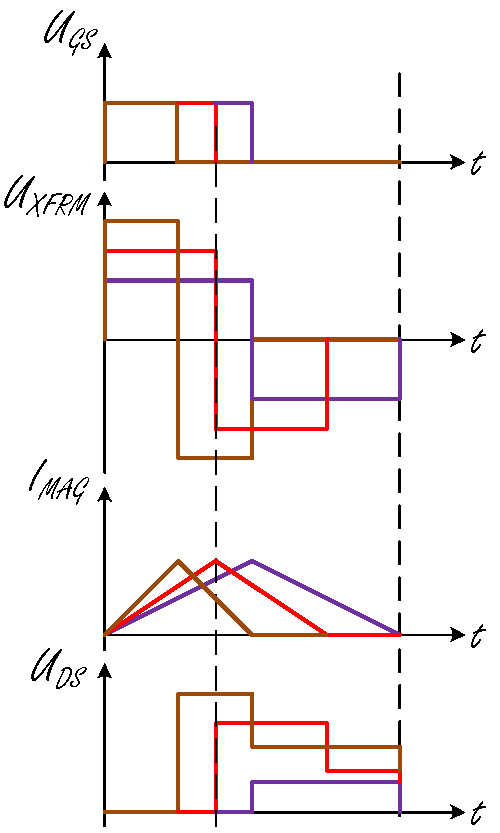
\includegraphics[width=0.5\linewidth]{imag_forward_converter.pdf}
    \caption[Magnetizační proud]{Vrcholová hodnota magnetizačního proudu je konstantní pro
             jakékoliv velikosti vstupního napětí, neboť regulační smyčka zajistí, aby napěťová
             plocha $V_{in}\cdot t_{on}$ byla konstantní}
    \label{enz:fig_imag_forward_converter}
    \end{figure}
    
    Pokud bychom měřili magnetizační proud primárního vinutí, dospěli bychom k průběhům na obr.
    \ref{enz:fig_imag_forward_converter}, jenž vykazují stejnou vrcholovou hodnotu pro různé hodnoty
    vstupního napětí. Je to dáno tím, že pokud měnič během měření pracoval v uzavřené regulační
    smyčce, bude součin $V_{in}\cdot t_{on}$ konstantní a za předpokladu, že magnetizační indukčnost
    je též neměnná, pak dle předchozí rovnice dospějeme $i_{mag_{max}} = konst$.
   
    %------------- Jednočinný propustný měnič s aktivním clampingem ------------------------------
  \subsection{Jednočinný propustný měnič s aktivním clampingem}\label{ENZ:kap_afwdconv}  
    Obecně pro všechny varianty  propustných měničů s transformátorem lze říci, že jsou vhodné pro
    přenos velkých výkonu. Je to dáno principem činnosti, kdy proud podílející se na přenosu výkonu
    se nepodílí na magnetizaci jádra transformátoru (teče v době $t_{on}$ a to jak na sekundární
    straně tak i na primární - kompenzace magnetických účinku). Může se proto zvyšovat, aniž by
    rostlo sycení jádra transformátoru. Toto sycení je určeno pouze integrálem primárního napětí a
    počtem primárních závitu. Lze proto zvýšením pracovního kmitočtu docílit zmenšení velikosti
    transformátoru, jak to bylo vysvětleno na konci kap. \ref{ES:kap_simple_rozbor_trafa}.
    \begin{figure}[ht!]
      \centering
      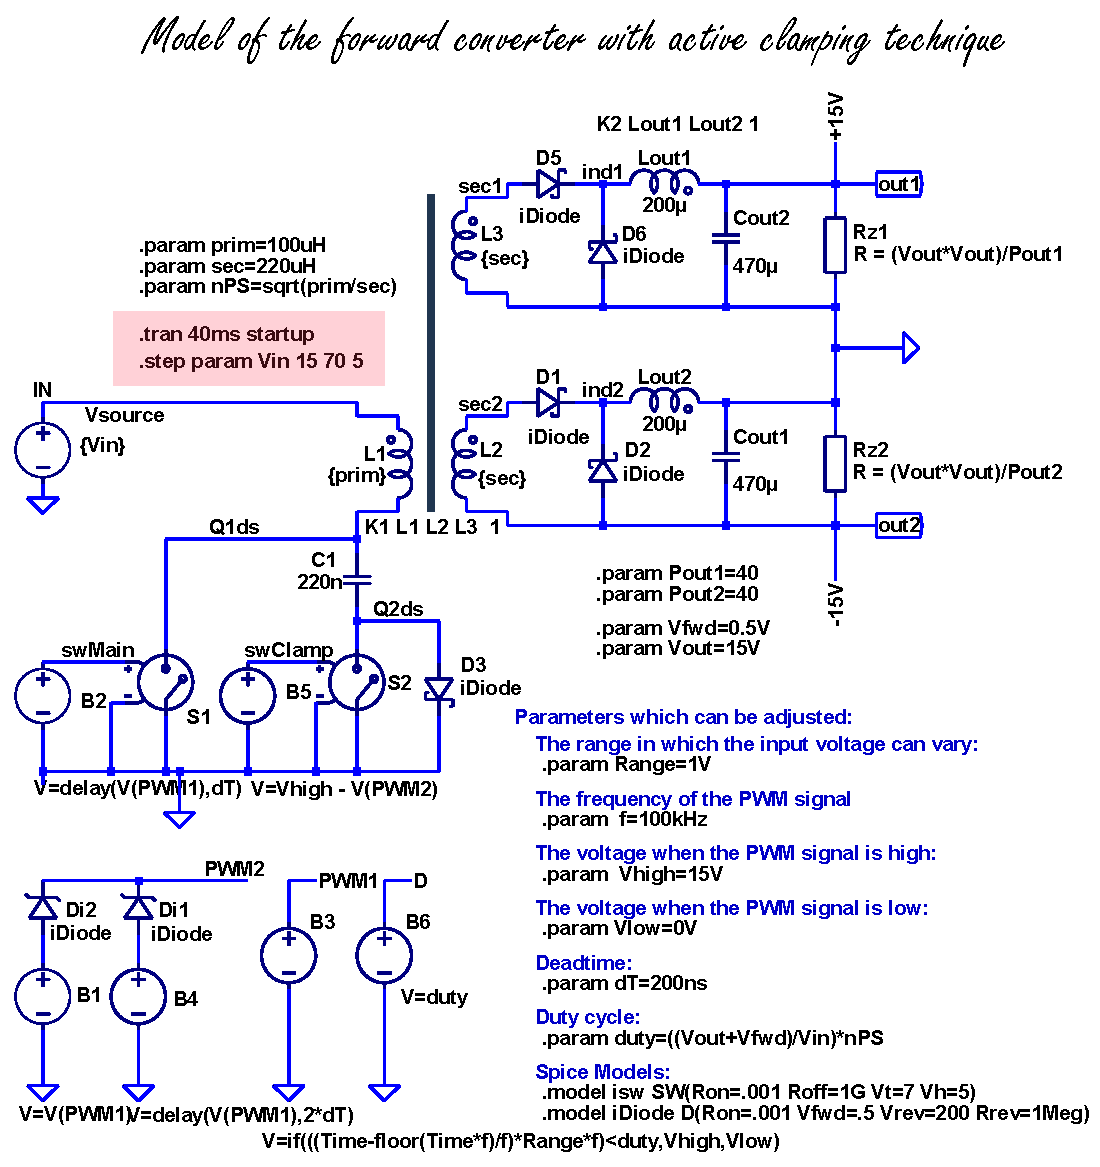
\includegraphics[width=\linewidth]{forward_converter_active_ltspice_model.pdf}
      \caption[Propustný měnič s aktivním clampingem]{Propustný měnič s aktivním clampingem}
      \label{enz:fig_imag_a_lt_frwd_conv}
    \end{figure}   


